\begin{figure*}[t]
    \centering
    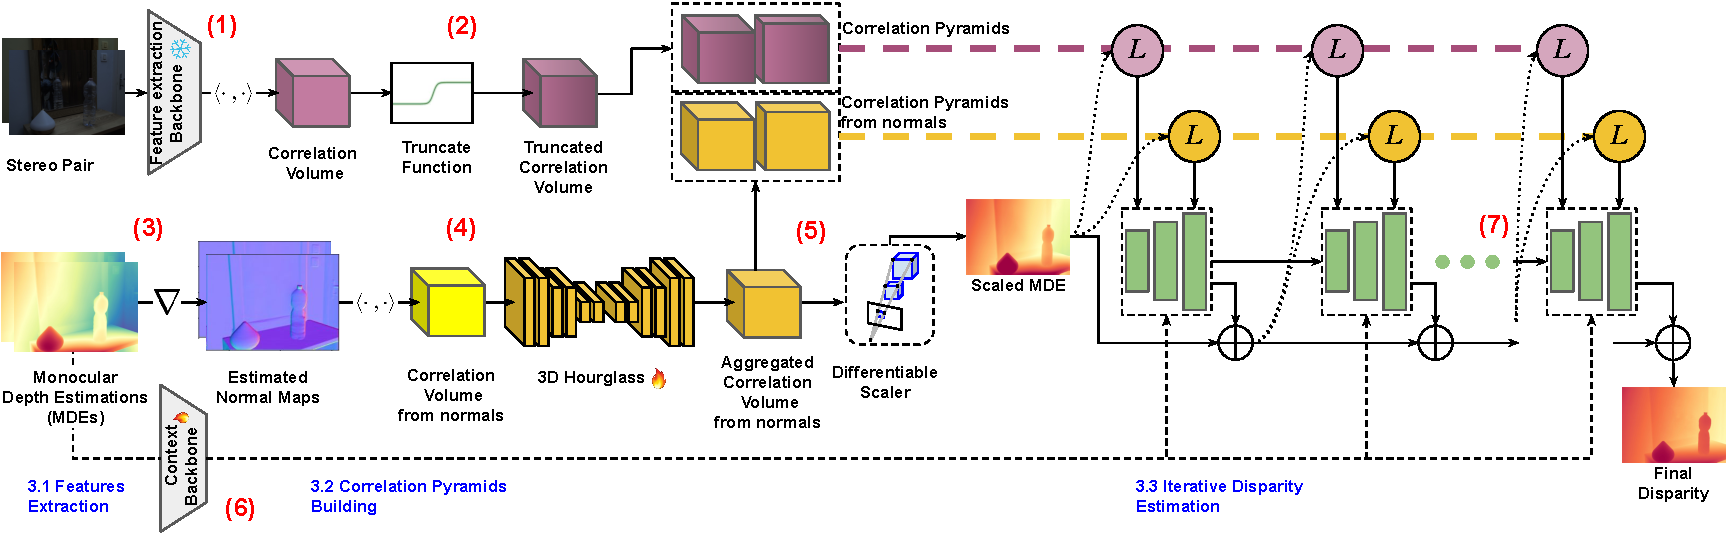
\includegraphics[width=0.98\linewidth]{imgs/final_arch_blin_con_numerini.pdf}\vspace{-0.2cm}
    \caption{\textbf{\method Architecture.} Given a stereo pair, \textcolor{red}{\bf(1)} a pre-trained backbone is used to extract features and then build a correlation volume. Such a volume is then truncated \textcolor{red}{\bf(2)} to reject matching costs computed for disparity hypotheses being \textit{behind} non-Lambertian surfaces -- glasses and mirrors. On a parallel branch, the two images are processed by a monocular VFM to obtain two depth maps \textcolor{red}{\bf(3)}: these are used to build a second correlation volume from retrieved normals \textcolor{red}{\bf(4)}. This volume is then aggregated through a 3D CNN to predict a new disparity map, used to align the original monocular depth to metric scale through a differentiable scaling module \textcolor{red}{\bf(5)} for it. In parallel, the monocular depth map from left images is processed by another backbone \textcolor{red}{\bf(6)} to extract context features.
    Finally, the two volumes and the context features from monocular depth guide the iterative disparity prediction \textcolor{red}{\bf(7)}.}
    \label{fig:arch}
\end{figure*}

\section{Related Works}
\label{sec:related}

We briefly review the literature relevant to our work.

    \textbf{Deep Stereo Matching.} In the last decade, stereo matching has transitioned from classical hand-crafted algorithms \cite{scharstein2002taxonomy} to deep learning solutions, leading to unprecedented accuracy in depth estimation. Early deep learning efforts focused on replacing individual components of the conventional pipeline \cite{zbontar2015computing,vzbontar2016stereo_MC-CNN,seki2017sgm, spyropoulos2014learning, tosi2024neural}. Since DispNetC \cite{mayer2016large}, end-to-end architectures have evolved into 2D \cite{yin2019hierarchical,liang2018learning_iResNet,song2019edgestereo, yin2019hierarchical} and 3D \cite{kendall2017end_GC-NET,yang2019hierarchical,zhang2019ga,bangunharcana2021correlate,Zeng_2023_ICCV,chang2018pyramid,guo2019group,shen2021cfnet,chen2023learning,shen2022pcw} approaches, processing cost volumes through correlation layers or 3D convolutions respectively. More recent advances, thoroughly reviewed in \cite{poggi2021synergies,laga2020survey,tosi2024survey}, include recurrent architectures for stereo matching~\cite{lipson2021raft,wang2024selective, chen2024mocha, zhao2023high, xu2023iterative, li2022practical, Jing_2023_ICCV, gong2024learning} inspired by RAFT~\cite{teed2020raft}, Transformer-based solutions \cite{Li_2021_ICCV_STTR, guo2022context_CEST, xu2023unifying, Su_2022_CVPR_Chitransformer, croco_v2,lou2023elfnet,zhang2024learning} for capturing long-range dependencies, and fully data-driven MRF models \cite{guan2024neural}. Among them, some methods specifically address temporal consistency in stereo videos \cite{Zhang2023TemporalStereo, Karaev_2023_CVPR, jing2024match, zeng2024temporally}. Domain generalization remains a major challenge, with various approaches proposed including domain-invariant feature learning \cite{zhang2019domaininvariant, Liu_2022_CVPR, Rao_2023_CVPR, Chuah_2022_CVPR, Song_2021_CVPR}, hand-crafted matching costs \cite{cai2020matchingspace, cheng2022revisiting}, integration of additional geometric cues \cite{aleotti2021neural, Pilzer_2023_WACV, tosi2024neural}, and exploitation of sparse depth measurements from active sensors \cite{poggi2019guided, bartolomei2023active, li2024stereo}. In parallel, self-supervised approaches \cite{godard2017unsupervised, Liu_2020_CVPR_Flow2Stereo} have emerged as effective alternatives to supervised learning, even using pseudo-labels from traditional algorithms \cite{tonioni2017unsupervised, aleotti2020reversing} or deploying neural radiance fields \cite{Tosi_2023_CVPR}. Despite the numerous attempts to improve specific aspects through the aforementioned techniques, recent architectures achieve remarkable generalization by combining their architectural advances with the increasing availability of diverse training data, while online adaptation techniques enable further improvements during deployment through self-supervised learning \cite{tonioni2019real, kim2022pointfix, poggi2021continual, Poggi_2024_CVPR}. However, although progress on challenges like over-smoothing \cite{Tosi2021CVPR_SMD,Xu_CVPR_2024_ADL} and visually imbalanced stereo \cite{liu2020visually,Chen_2022_CVPR,aleotti2021neural,tosi2024neural}, handling non-Lambertian surfaces remains particularly challenging due to limited annotated data and complex appearance, with rare works like Depth4ToM \cite{costanzino2023learning} specifically addressing this through semantic guidance. Among all the aforementioned approaches, there have been limited attempts to integrate stereo with monocular cues \cite{Chen_2021_ICCV, aleotti2020reversing, watson2020learning}, mostly in self-supervised settings or through loose coupling between modalities.
    
    \textbf{Monocular Depth Estimation.} Parallel to developments in stereo matching, single-image depth estimation has evolved from hand-crafted features~\cite{Saxena2008} to deep learning methods~\cite{chen2016single, eigen2014depth, laina2016deeper, Ramamonjisoa_2020_CVPR, wang2020cliffnet}, with self-supervised approaches~\cite{godard2017unsupervised, zhou2017unsupervised, mahjourian2018unsupervised, godard2019monodepth2, poggi2018learning, watson2019depthhints, zhao2022monovit}  reframing the task as an image reconstruction problem. This led to multi-task approaches incorporating flow~\cite{zou2018df, yin2018geonet, ranjan2019competitive, tosi2020distilled} and semantics~\cite{zama2019geometry, guizilini2020semantically}, alongside advances in uncertainty estimation~\cite{poggi2020uncertainty, hornauer2022gradient} and dynamic object handling~\cite{klingner2020self, sun2023dynamodepth, moon2023ground}.
    Affine-invariant models~\cite{Ranftl2022, Ranftl2021, Yin2020, Eftekhar2021} marked a breakthrough in cross-domain generalization, pioneered by MiDaS~\cite{Ranftl2022} and followed by works like DPT~\cite{Ranftl2021} and, more recently, the Depth Anything series \cite{depth_anything_v1}. These approaches used different data sources, from internet photos~\cite{li2018megadepth,Yin2020,Spencer2023c,Spencer2024} to car sensors~\cite{geiger2012we,menze2015object} and RGB-D devices~\cite{Silberman2012, Cho2021}, representing the first generation of VFMs for monocular depth estimation. Recent works have focused on metric depth estimation through camera parameter integration~\cite{Yin2023, hu2024metric3dv2,Guizilini2023}, diffusion models~\cite{Ji2023, Duan2023, Saxena2023, Saxena2023b, ke2023repurposing, fu2024geowizard}, and temporal consistency~\cite{shao2024learning, hu2024depthcrafter}.
    Moreover, material-aware methods~\cite{costanzino2023learning}, diffusion models~\cite{tosi2024diffusion}, and large-scale synthetic datasets have enabled robust monocular depth estimation for non-Lambertian surfaces~\cite{depth_anything_v2}. Stereo methods, however, still struggle with these surfaces due to limited real-world and synthetic annotated data, affecting generalization. We address this by integrating robust monocular VFMs into a stereo architecture.

